\chapter*{\large\textsf{Statistiken}}
        \thispagestyle{empty}

Bei einem Buch handelt es sich auch immer um einen linguistischen Korpus. Schon
das Wort \emph{Korpus} deutet an, dass durch diese Umbenennung aus einem
lebendigen Text voller Feen und Elfen eine Tote Liste aller enthaltener Wörter
gemacht wurde. Und solche Listen ziehen Statistiker an, die dann anfangen
Erbsen und alle anderen Wörter zu zählen.

Wie so oft bei Wissenschaft, ist das Ergebnis erwartbar. Auf den ersten Plätzen
rangieren:

\begin{enumerate}
    \item die (1'021)
    \item und (989)
    \item sie (661)
    \item der (582)
    \item das (476)
    \item zu (415)
    \item nicht (387)
    \item es (363)
    \item aber (350)
    \item er (350)
\end{enumerate}

Wenn man Menschen glaubt, die solch absurdes Zählen zu ihrem Beruf gewählt
haben, ist es nicht Schreibfaulheit, die so viele kurze Wörter in die Charts
gebracht hat, sondern das ist so üblich. Wie Ameisen: klein, aber viele.

Das erste Subsatntiv ist auf Platz 71 die \emph{Maus}, dann auf Platz 88
\emph{Menschen} und genau auf Platz 100 \emph{Mama}. Das grosse \emph{M} hat
klar das Rennen für sich entschieden. Konkurrenzlos drei Mal in den Top\,100.
Die oben genannte \emph{Fee} landet auf Platz 500 und auf Platz 1'000 ist
\emph{Schönheit}. Na ja, es steht an tausendster Stelle in der Liste, mit zwei
Nennungen gibt es aber noch sehr viele andere Wörter auf dem Platz, der
tatsächlich der 112te ist.

Im Grunde gibt es aus der quantitativen Linguistik nur eine mir bekannte
interessante Erkenntnis. Die Verteilung der Ranghäufigkeit (Wie oft kommt das
häufigste Wort vor, wie häufig das Zweithäufigste usw.) folgt einer Verteilung,
die nach ihrem Entdecker Zipf benannt ist. Klingt wie aus einem Wilhelm Busch
Buch. Und diese Zipf'sche Verteilung folgt einer Reihe mit noch mehr Wohlklang,
der harmonischen Reihe
$\left(\frac{1}{1},\frac{1}{2},\frac{1}{3},\dots\right)$ beschrieben
werden. 

Es gibt jetzt also die theoretische Verteilung der Wörter und die tatsächliche
in diesem Buch. Plotten wir beide zusammen ergibt sich eine Grafik wie in
Abbildung \ref{dend1}. Ein Statistiker sagt dann, die Übereinstimmung ist \emph{ganz
okay}.

\begin{figure}[ht]
\centering
	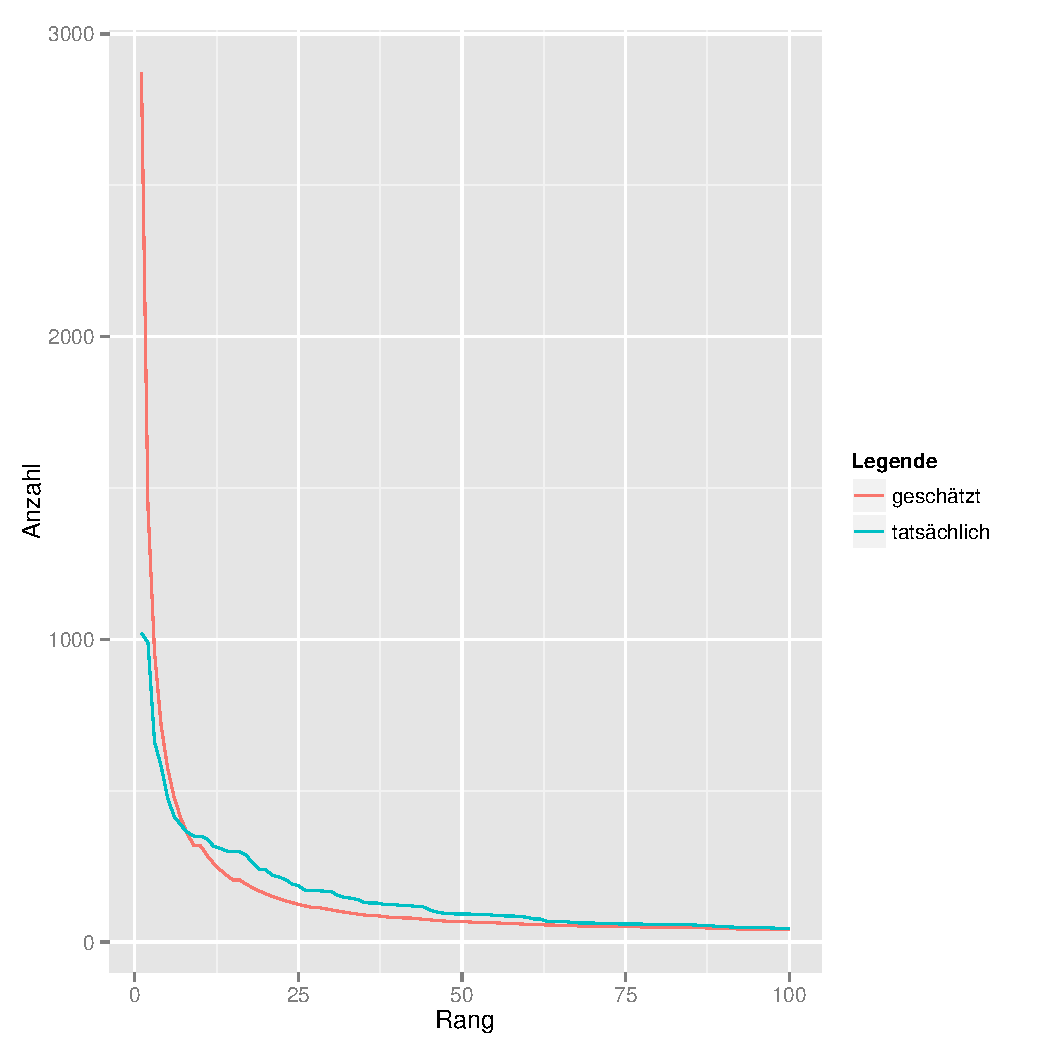
\includegraphics[height=.6\textheight,width=\textwidth]{tinaStat/zipfAlle.pdf}
	\label{dend1}
\end{figure}
